\documentclass[border=4pt]{standalone}
% Preámbulo común de las figuras. Cada figura es un documento standalone
% que se compila a SVG con scripts/build_figures.sh
\usepackage[utf8]{inputenc}
\usepackage{amsmath}
\usepackage{tikz}
\usepackage[american, siunitx]{circuitikz}
\usetikzlibrary{arrows.meta,calc,decorations.pathmorphing,patterns}
\tikzset{
  >={Stealth[length=2.2mm]},
  eje/.style={->, thin},
  hilo/.style={thick},
}
% Paleta común: tonos medios legibles sobre fondo claro
\definecolor{azul}{RGB}{31,94,168}
\definecolor{rojo}{RGB}{192,57,43}
\definecolor{verde}{RGB}{39,128,73}
\definecolor{naranja}{RGB}{211,120,30}
\definecolor{morado}{RGB}{125,60,152}

\begin{document}
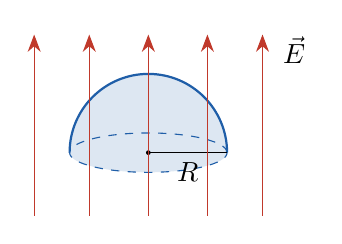
\begin{tikzpicture}[scale=1.0]
  \fill[azul!15] (-1,0) arc (180:0:1) arc (0:-180:1 and 0.25);
  \draw[azul, thick] (-1,0) arc (180:0:1);
  \draw[azul, dashed] (0,0) ellipse (1 and 0.25);
  \draw (0,0) -- node[below]{$R$} (1,0);
  \fill (0,0) circle (0.03);
  \foreach \x in {-1.45,-0.75,0,0.75,1.45} \draw[->, rojo] (\x,-0.8) -- (\x,1.5);
  \node at (1.85,1.3) {$\vec E$};
\end{tikzpicture}
\end{document}
